2次元物体の定常状態の温度分布の解析に関して、
ガウス・ザイデル法による数値解析プログラムをソースコード\ref{s1}に示す。また、分割数が6の場合と12の場合の実行結果を図\ref{j1}、図\ref{j2}に示す。
\begin{lstlisting}[caption=ガウス・ザイデル法による数値解析プログラム,label=s1]
#include <stdio.h>
#include <stdlib.h>
#include <math.h>
  
int N; // メッシュ数
float L;// 正方形の辺の長さ
#define Tm 50
#define dx (L / N) // メッシュの間隔
#define dy (L / N)
#define T0 0.0     // 境界条件1
//#define T1 10.0  // 境界条件2 → sin関数
#define T2 0.0     // 境界条件3
#define T3 0.0     // 境界条件4
#define eps 1e-5   // 収束判定の閾値
  
  
int main()
{
  printf("width? [m]: ");
  scanf("%f", &L);
  printf("mesh?: ");
  scanf("%d", &N);
  int i, j;
  int ITER = 0;
  double T[N+1][N+1] = {0}; // 未知数の温度分布
  double T_true[N+1][N+1] = {0}; 
  double diff = eps + 1.0; // 収束判定の差分(1回目のループ条件を満たすための初期化)

  //境界条件の設定
  for (i = 0; i < N+1; i++) {
    T[i][0] = T0;   // 左辺
    T[i][N] = T2; // 右辺
  }
  for (j = 0; j < N+1; j++) {
    T[0][j] = Tm*sin((M_PI/L)*j*dx);// 上辺
    T[N][j] = T3; // 下辺
  }

  // ガウスザイデル法の反復
  while (diff > eps) {
    diff = 0.0;
    for (i = 1; i < N; i++) {
      for (j = 1; j < N; j++) {
        double T_old = T[i][j];
        T[i][j] = 0.25*(T[i+1][j] + T[i-1][j] + T[i][j+1] + T[i][j-1]);
        diff += fabs(T[i][j] - T_old); //1サイクル分の誤差
      }
    }
    ITER++;
  }
 
  // 厳密解
  for (i = 0; i < N+1; i++) {
    for (j = 0; j < N+1; j++) {
        T_true[i][j] = Tm/sinh(M_PI)*sin(M_PI/L*j*dx)*sinh(M_PI/L*i*dy);
    }
  }
 
  // 結果の出力
  printf("Result:  Gauss-Seidel Approximate Solution (Exact Solution)\n");
  printf("Cycle: %d\n", ITER);
  for(i = 0; i < N+1; i++){
    for (j = 0; j < N+1; j++) {
        printf(" %f  ", T[i][j]);
    }
    printf("\n");
    for (j = 0; j < N+1; j++){
          printf("(%f) ", T_true[N-i][N-j]);
    }
    printf("\n");
  }
  return 0;
}
\end{lstlisting}

\begin{figure}[H]
  \begin{center}
  \subfigure[分割数:6]{
  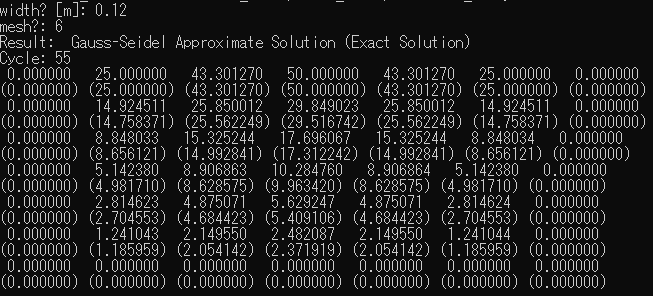
\includegraphics[width=\columnwidth]{img/1.png}
  \label{j1}
  }
  \subfigure[分割数:12]{
  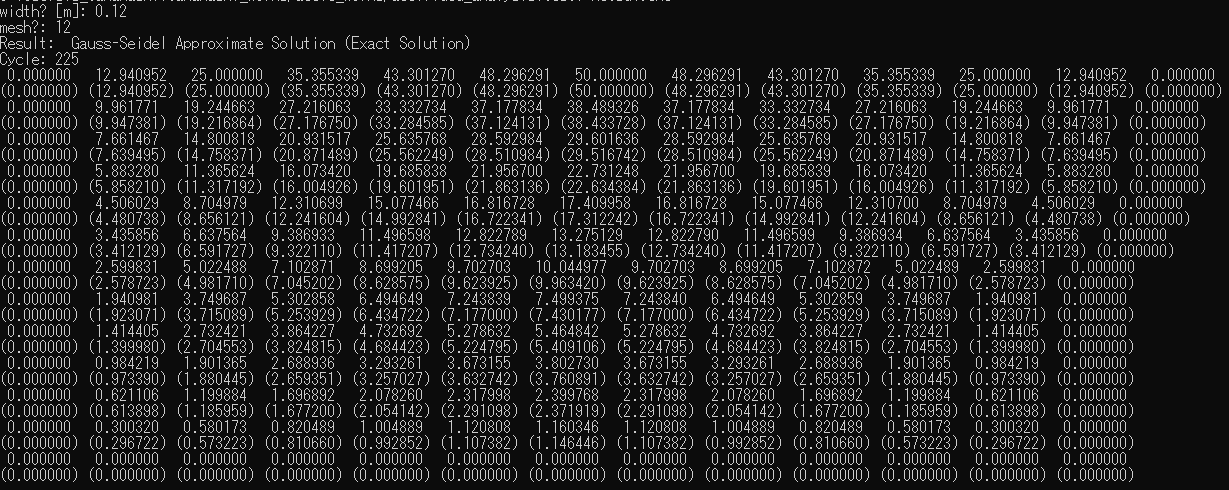
\includegraphics[width=\columnwidth]{img/2.png}
  \label{j2}
  }
  \caption{実行結果}
  \label{im1}
  \end{center}
\end{figure}